\documentclass[11pt,a4paper]{jsarticle}                    % fir platex
%\documentclass[11pt,a4paper,uplatex]{ujreport} 	% for uplatex
%
\usepackage{amsmath,amssymb}
\usepackage{bm}
\usepackage{graphicx}
\usepackage{ascmac}
\usepackage{float}
\usepackage{here}
\usepackage{listings,jvlisting}
%
\lstset{
  basicstyle={\ttfamily},
  identifierstyle={\small},
  commentstyle={\smallitshape},
  keywordstyle={\small\bfseries},
  ndkeywordstyle={\small},
  stringstyle={\small\ttfamily},
  frame={tb},
  breaklines=true,
  columns=[l]{fullflexible},
  numbers=left,
  xrightmargin=0zw,
  xleftmargin=3zw,
  numberstyle={\scriptsize},
  stepnumber=1,
  numbersep=1zw,
  lineskip=-0.5ex
}

\setlength{\textheight}{40\baselineskip}
\addtolength{\textheight}{\topskip}
\setlength{\voffset}{-0.2in}
\setlength{\topmargin}{0pt}
\setlength{\headheight}{0pt}
\setlength{\headsep}{0pt}

\setlength{\textwidth}{\paperwidth}     % ひとまず紙面を本文領域に
\setlength{\oddsidemargin}{-5.4truemm}  % 左の余白を20mm(=1inch-5.4mm)に
\setlength{\evensidemargin}{-5.4truemm} % 
\addtolength{\textwidth}{-40truemm}     % 右の余白も20mmに
%
\newcommand{\divergence}{\mathrm{div}\,}  %ダイバージェンス
\newcommand{\grad}{\mathrm{grad}\,}  %グラディエント
\newcommand{\rot}{\mathrm{rot}\,}  %ローテーション
%
\title{脳を学ぶ上で重要な数学シリーズ 計算論編}
\author{後藤 優仁}
\date{\today}
\begin{document}
\maketitle
%
%
\tableofcontents

\section{はじめに}
さて,この数学シリーズの中でもこのadvancedはかなり異質で,筆者が脳神経科学を研究する上で関わっていった様々な (あまり一般的ではない) 議論を展開するために必要になった数学的知識をまとめる場です.筆者は脳活動の非線形ダイナミクスの機能的な役割を研究しています.脳は多数の非線形素子が結合した大自由度の力学系とみなすことができ,多様なダイナミクスを示します.計算論的神経科学の観点で,神経系が示す同期,自発活動,誘発活動ダイナミクス,ノイズ誘発同期,...といった様々な現象を捉え,その情報処理メカニズムの解明を試みています.\\
\\
 こうした作業には,信号処理は勿論,非線形ダイナミクス(つまり力学系),情報理論,複雑系,機械学習...多種多様な数学的,理論的知識が求められます.この勉強については終わりがなく,本当に役に立つのかも分かりません.ただ確実に言えるのは,\\
\\
「○○をやっている時の脳は△△領域で~~ ms後に × Hzの波が同期している!!」
\\
\\
なんてことだけ見ていても,脳を理解する事は出来ないということです.その活動が何故大事なのか,その活動を通してどんな処理をしているのか...こうしたところまで理解してこその科学だと,筆者含め計算論的神経科学者たちは考えています.\\
\\
実験的にデータを集めるだけでは理解に至らず,その背景で何が行われているのか,どんな表現がなされているのか.そんなところまで考えないとだよね,というスタンスです.その必要性が分からん,そんなに大事だろうか.そう思う人はユニークな思考実験的論文があるので是非読んでみてください\cite{radio}\cite{Jonas}.
\\
何をもって脳の理解とするか?
\\
この問に答えるのが,有名なマーの3レベルという概念?お話?\cite{mar}です.\\
\begin{itemize}
 \item{計算理論}
 \item{表現とアルゴリズム}
 \item{ハードウェアによる実装}
\end{itemize}

この3段階を踏み,相互に対応付ける事が脳の理解に大切だ,とする話です.計算理論は,我々が脳を使ってどんな「計算」を行っているのか,行っているべきなのか,といった議論.自由エネルギー原理だとかの話,すなわち脳が採用している戦略を考える所です.ハードウェアによる実装は,多くの神経科学者がやっているように脳のどの部分でどんな活動が起きていてといった解剖学・生理学的知見.最後に表現とアルゴリズムは,ハードウェアの実装を使っていかに計算理論で提案された処理を実行するのか,になります.\\
\\
彼に言わせれば,これまで主流の神経科学はハードウェアの実装ばかりだったわけですね.計算理論と表現に関する議論は,無論ありましたがあまり活発ではなかった.
\\
\\
ここから先,どう考えるかは個人の自由だと思います.計算理論や表現についても考えていこうとするか,そんなに色々手を出しても回収しきれないと見切りをつけるか,あるいは他の人が結び付けてくれる事を期待して実験データを提供するに集中するのか...\\
\\
筆者は,計算理論と実装を結ぶ,表現の研究者になりたいと考えた次第です.一番勉強する事が多いような気もしますが,楽しんでやっていきます.\\
\\
長くなりましたが,本書はそんなモチベーションのもと,計算理論やアルゴリズムについて学習したことをまとめていくものにします.なので神経に本当に役立つのか,理解が正しいのか,様々な問題があると思いますが,まあ教科書ではなく筆者のノートだと思って見てください.結構やってみると楽しいです.また本稿はその性質上,随所で本や論文を引用しながら議論を展開していきます.筆者の拙い理解での説明では不十分だったり不適切だったりすることも少なくないはずなので,気になるところは適宜参照してください.\\

\section{情報理論}
近年は神経科学に情報理論の議論を輸入するのが流行りになっている気がします.脳波の解析もだし,情報処理の理論もそうだし,いろんなとこで見るのでとりあえず勉強.関係する研究は以下とか\\
\begin{itemize}
 \item{自由エネルギー原理\cite{fep}}
 \item{Phase Amplitude Couplingの評価. \cite{tort}}
 \item{相互情報量}
 \item{トランスファーエントロピー}
\end{itemize}
*まだちゃんと引っ張ってきてない
\subsection{エントロピー}
はじめにエントロピーの考え方を導入しましょう.まずは離散確率変数$x$を考えます.観測者がこの変数に対するある値を観測したとき,どれだけの情報量,surpriseを得られるのか.これを考える概念がエントロピーです.\\
直観的に,起きそうもない事象が得られたら情報量は大きいし,その逆も然りですよね.宝くじで1等があたるのはめちゃくちゃびっくりする,つまり情報量大きいけど,参加賞的なのもらっても何も思いません.つまり情報量は確率分布$p(x)$に依存していて,その値によって定まる単調な関数$h(x)$といえます.\\
\\
また,2つの事象$x, y$を考えたとき,これらが独立なら両方を観測したときの情報量は別個に観測したときの情報量の和と等しい(式\ref{eq:sum})はずです.宝くじが当たる事によるsurpriseによって,帰りに頭に雷が落ちてくる事によって生じるsurpriseが小さくみたいになることはないですよね?あるかもな.ないって事にしてください.\\
よって以下の式(\ref{eq:sum})が成り立ちます.
\begin{eqnarray}
\label{eq:sum}
h(x,y) = h(x) + h(y)
\end{eqnarray}

次に,これらの事象の同時確率についても単純に積で求められます(式\ref{eq:product}).宝くじが当たり,かつ頭に雷が降ってくる確率です.

\begin{eqnarray}
\label{eq:product}
p(x,y) = p(x)p(y)
\end{eqnarray}

もし式(\ref{eq:sum}, \ref{eq:product})が分からないようなら基本的な確率が出来てないので,statistics.pdfで勉強してみてください.\\
\\
さて,ここはちょっとテクいです.\\
\\
この二つの関係から,xとyの確率をかける操作をしたものに対して何らかの処理をしたものが,何らかの処理をしたxとyの和になっているので,関数$h(・)$は対数をとっている事が分かり(ほら,掛け算って対数だと足し算じゃん?),

\begin{eqnarray}
h(x) = -log p(x)
\end{eqnarray}
がいえます.log (x)は単調増加で,確率p(x)は常に0から1の範囲をとるため,$h(x)$の値を常に正にするため符号を反転させている事に注意です.ここで対数の底に2を採用するのが情報理論での一般の使い方で,その場合は$h(x)$の単位はbitになるようです.\\
これを使って,信号のサイズ,情報量(bit)を算出してるわけですね.あとデータの圧縮なんかにも関係するぽいですがそこまでは知らないし触れませんし触れられません.\\
\\
次に,この値を分布全体に適用する事を考えます.つまり,確率分布そのものが与える情報量です.その指標として,確率変数$x$の分布$p(x)$に関して$h(x)=-log p(x)$の期待値をとることで,情報量の平均を定義します.確率変数の期待値の一般的な計算です.これも分からなければやはりstatisticsに行ってください.\\

\begin{eqnarray}
\label{eq:entropy}
H[x] = - \Sigma_{x} p(x) log p(x)
\end{eqnarray}

式(\ref{eq:entropy})に定義する量をシャノンエントロピーといいます\cite{prml}.意外と簡単ですね.もっと難しいと思ってました.\\
\\
ついでにこれを連続変数にすると微分エントロピー(式\ref{eq:entropy2})が求まります.

\begin{eqnarray}
\label{eq:entropy2}
H[x] = - \int p(x) log p(x) dx
\end{eqnarray}

言うまでもないと思いますが,$ \Sigma_{x} p(x)$ も$ \int p(x)$も1です.\\
さて,次に当然浮かぶ疑問は,どんな確率分布だとどんなエントロピーが算出されるのか,です.\\
ちゃんと数学的に証明することも出来るっぽいけど面倒だしそこにあんま興味ないので,simulationしてみます.\\

とりあえず一様分布で確認してみます.0.1から1の値をとる,サンプル数10の一様分布(図\ref{im:ent1})のエントロピーを算出します(コード\ref{sc:ent1}).
\begin{lstlisting}[caption=エントロピーの計算,label=sc:ent1]
x = [0.1:0.1:1];
px = zeros(1,10)+0.1;
H = - sum(x .* log(px));

\end{lstlisting}

\begin{figure}[H]
\label{im:ent1}
  \centering
  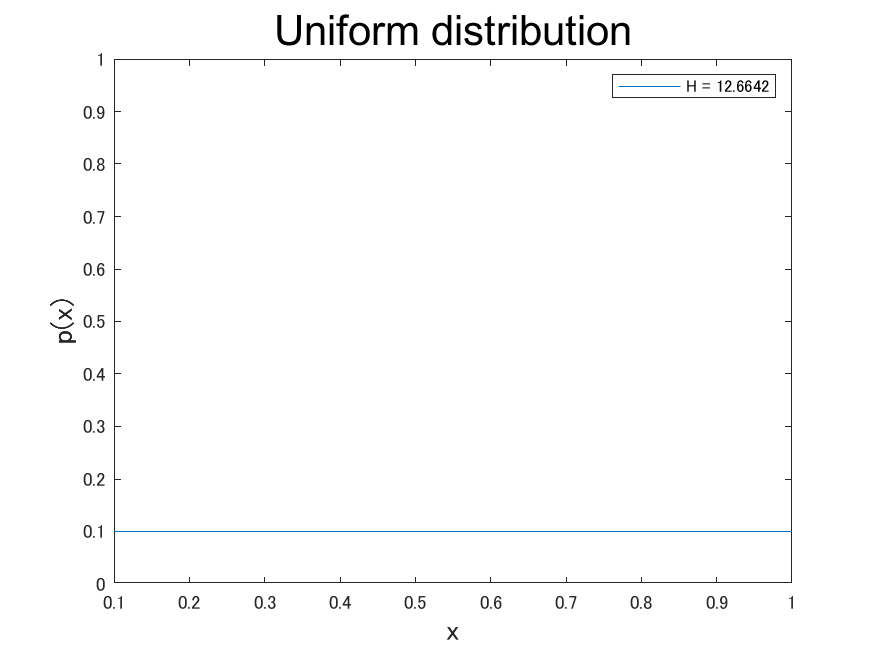
\includegraphics[width=200mm, bb=0 0 600 400]{../figures/dis_entropy1.png}
  \caption{0.1が10この一様分布}
\end{figure}

エントロピーは12.7でした.次に,同じ一様分布でもサンプル数が多いとどうなるのか試します.先ほどと同じ条件の,100個のデータ(図\ref{im:ent2})です.

\begin{figure}[H]
\label{im:ent2}
  \centering
  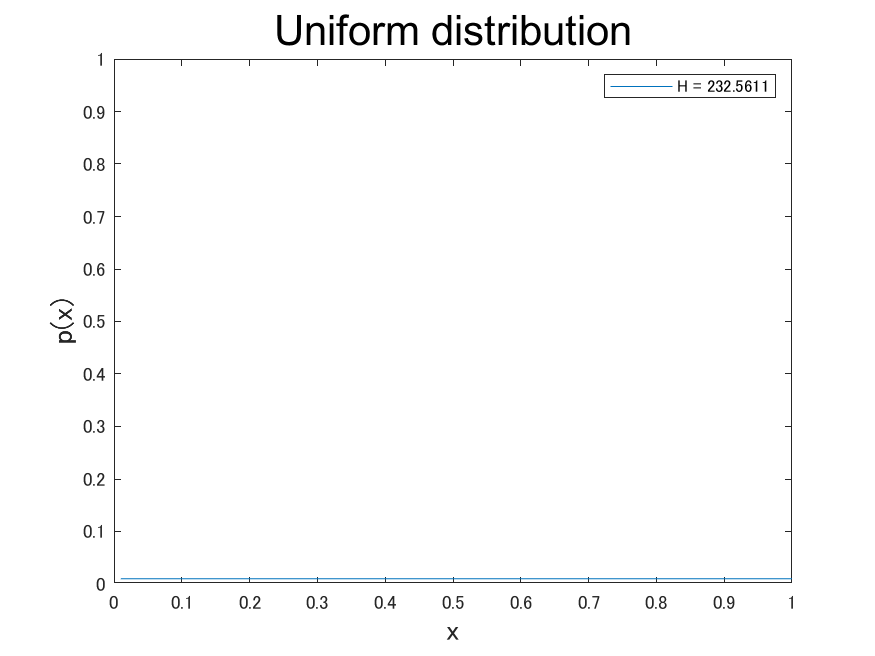
\includegraphics[width=200mm, bb=0 0 600 400]{../figures/dis_entropy2.png}
  \caption{0.01が100この一様分布}
\end{figure}

エントロピーは232.5. 大きくなりましたね.データ数に応じてエントロピー自体は大きくなるぽいです.\\
次に山を持たせた分布で見てみます.

\begin{figure}[H]
\label{im:ent2}
  \centering
  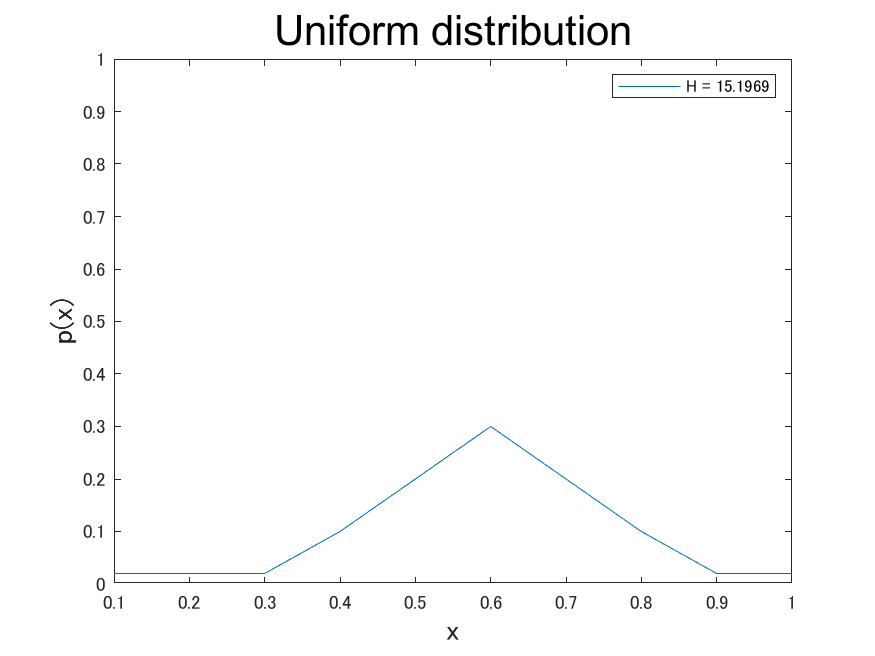
\includegraphics[width=200mm, bb=0 0 600 400]{../figures/dis_entropy3.png}
  \caption{適当につくった山あり分布}
\end{figure}

エントロピーは22.3.一様分布に比べるとかなり小さいです.本当はもっと山の位置動かしたり急峻にさせてみたりと比較したいですが,飽きたので結論.(離散)エントロピーは確率分布$p(x)$が一様分布に近付く程大きくなり,一様分布の時に最大になります.$x * log(x)$なのでまあ,考えればそうかなって感じ.証明は結構めんどくさいぽいです.\\
この性質から,状態の予測が困難であるほどエントロピーが高い事になるので,不確かさ(Uncertainty)の指標として用いられる事が多いですよね.\\
\\
ちなみに微分エントロピーの場合はガウス分布が最もエントロピー高いようです.\\
\\
他にも見れる性質があって,まず$p(x)$が0は困ります.logにかけた時に計算がこわれるので.無限に吹っ飛びます.\\
\\
あと,一様分布の比較から分かるようにデータ数が多いほどエントロピーも増大するぽいですね.これもまあ普通に総和とってるんだから当たり前か?

\subsection{KL距離}
さて,このエントロピーがどんな事に使えるのか考えていきます.エントロピーは分布の特徴を表す量になっていたわけなので,これを使うと二つの分布の比較,なんてことも出来ることになります.直観的には,全く同じ特徴の分布同士ならそのエントロピーに差はないし,違う分布なら差がある,という感じです.\\
\\
式にしてみましょう.まず,微分エントロピー($- \int p(x) log p(x)$)は確率変数xの分布$p(x)$の元での期待値でした.なら,ここで新しい分布$q(x)$を考えたとき,仮にこの分布が同一($p(x) = q(x)$)であれば,

\begin{eqnarray}
\label{eq:KL1}
  \int p(x) log q(x)dx - \int p(x) log p(x)dx= 0
\end{eqnarray}
が成り立つ事になります.同じ分布の元で考えた同じ確率変数の期待値だから,当たり前です.分布$p(x)$の元で見た$q(x)$の期待値が,分布$p(x)$の元で見た$p(x)$の期待値と等しい,ということです.逆にこの分布が異なるものであるほど,この計算の結果は大きな値を取る事になります.\\
\\
てなわけで,この量をちゃんと正負の調整した上で,「分布$p(x), q(x)$の相対エントロピー,あるいはカルバック-ライブラー距離,またはカルバックライブラーダイバージェンス」として以下の式で定義します\cite{prml}.

\begin{eqnarray}
\label{eq:KLD}
  \mathbb{D}_{KL}(p||q) = - \int p(x) log q(x)dx - (-\int p(x) log p(x)dx)\\
  = -\int p(x) log \frac{q(x)}{p(x)} dx
\end{eqnarray}

一寸ややこしく見えますが,基本的には式(\ref{eq:KL1})をlogについて整理しただけです.\\簡単ですね.\\
\\

KL距離の性質ですが,まず$\mathbb{D}_{KL}(p||q) \geq 0$です.距離だし.\\
等号が成り立つのは分布$p(x), q(x)$が等しいときのみです.\\
\\
それから$\mathbb{D}_{KL}(p||q) \neq \mathbb{D}_{KL}(q||p)$なことにも気を付けてください.分布$p(x)$の元で見た$q(x)$の期待値と, 分布$q(x)$の元でみた$p(x)$の期待値とは別物ですからね.\\
\\
それから,対数なのでKLDは以下のような表記のこともあります.一緒です.logの計算の性質を思い出してください.割り算は引き算です(?)

\begin{eqnarray}
\label{eq:KLD}
  \mathbb{D}_{KL}(p||q) =  \int p(x) log \frac{p(x)}{q(x)} dx
\end{eqnarray}
\\
留意してください.\\
\\
あと,KL ``距離''と日本語で呼んでいますが厳密には距離じゃないので注意が必要です.というのも,KLDは以下に示す距離の公理\cite{distance}を満たしていないからです.\\
\\

\begin{screen}
距離の公理\\
2点A,Bが与えられたとき, 実数$d(A,B)$を与える規則で, 次の性質を満たすものを距離という.
\begin{itemize}
\item{$d(A, B) \geq 0$}
\item{$d(A, B) = 0 \leftrightarrow A=B$}
\item{$d(A, B) = d(B, A)$}
\item{$d(A, B) + d(B, C) \geq d(A, C)$}
\end{itemize}
\end{screen}

このうち,KLDが満たしていないのはなんでしょう?\\
そう,3つめの対称性ですね!$\mathbb{D}_{KL}(p||q) \neq \mathbb{D}_{KL}(q||p)$でした.\\
\\
あと4つ目,三角不等式も怪しいと思うんですよね.呼んでた資料とかでは特に対称性のとこだけネチネチと言われてましたが,三角不等式はどうなんでしょう?\\
\\
直観的には微妙だと思ってて,だからKLDの値を単純に比較したりだとかの議論は出来ない気がしている.\\
\\
じゃあKLDはどう使うんだよって話ですが,最小化したい量として導入してるのが多い気がします.\\
つまり,予測分布を真の分布に近づけたい,だとかですね.この時に最小化する,分布と分布との距離として使われる量です.\\
あとは,一様分布と得られたデータ分布との距離を測る,なんて使い方もありました\cite{tort}. この場合は正規化的なのして,$\mathbb{D}_{KL}(P||U)$(where U is the uniform dist)を0-1の値にして使ってましたね.\\
\\
\\
いまのとこ個人的に分からないのは,$\mathbb{D}_{KL}(A||B)$と$\mathbb{D}_{KL}(C||D)$の値を比較した議論(たとえば,A-BはC-Dの3倍離れている!)なんてのは出来るのかなってところです.\\
ユークリッドなら自明に出来ると思うんですけど,これだとなんか出来ない気がする.三角不等式も怪しいし.\\
どうなんでしょう?今後の課題になってます.\\
\\

余談ですが,式(\ref{eq:KLD})の右辺第一項,$- \int p(x) log q(x)dx$は交差エントロピー$H(p,q)$とも言います.分布$p(x)$の元で見た$q(x)$の期待値なので,$p(x)$の分布を想定したとき,$q(x)$がどれだけ予測しにくいかとも捉えられます.\\
\\
これだけでも,交差エントロピー$H(p,q)$は正解値と推定値の比較なんかの用途で使えるようです.\\
\\
じゃあKLDと何が違うのか,というと,ここからは個人的な予想ですが...\\
問題なのは$p(x)$自体の分布が既にもってる情報量,つまり$H(p)$なんだと思います.\\
交差エントロピーは計算式をみれば分かるように,$p(x)$自体のエントロピーの影響を受けた数値になってしまうため,なんというか「どれくらい外れているか」の指標に使うにはフェアじゃない気がします.\\
\\
なので交差エントロピーの値から,$p(x)$自体が持っているエントロピーの値を差し引いた量が知りたいわけですね.そうすると式(\ref{eq:KLD})は
\begin{eqnarray}
\mathbb{D}_{KL}(p||q) = H(p,q) - H(p)
\end{eqnarray}
とも捉えられますね.あってるのかな?

\subsubsection{他の分布間距離}
確率分布同士の距離を測る指標は$\mathbb{D}_{KL}$だけでなく,他にも以下のようなのがあるっぽいです\cite{dist}.
\begin{screen}
\begin{eqnarray}
\chi^2(Q||P) := \Sigma_{i=1}^k \frac{(p_i - q_i)^2}{p_i} \qquad \qquad  \text{$\chi^2$統計量}\\
L_1(Q||P) := \int |Q(x) - P(x)|dx   \qquad \qquad  \text{$L_1$ノルム} \\
L_2(Q||P) := \int\{ Q(x) - P(x)\}^2 dx   \qquad \qquad  \text{$L_2$ノルム}\\
I_K(Q||P) := \int \{ \sqrt{Q(x)} - \sqrt{P(x)} \}^2 dx    \qquad \qquad  \text{ヘリンジャー距離}\\
\mathbb{D}(Q||P) := \int f(\frac{Q(x)}{P(x)}) Q(x)dx   \qquad \qquad  \text{f-ダイバージェンス}\\
I_\lambda(Q||P) := \int \{ (\frac{Q(x)}{P(x)})^{\lambda} -1 \}Q(x) dx   \qquad \qquad  \text{一般化情報量}\\
\mathbb{D}_{KL}(Q||P) := \int log(\frac{Q(x)}{P(x)})Q(x) dx   \qquad \qquad  \text{KL情報量}
\end{eqnarray}
\end{screen}
どれがどんな時にどう使われるとかは調べてないです,でもこれでいくと上3つはよく見る気がする.でもまあ全体的に似てるポイですね.なんとなく哲学というか考え方はどれも似たりよったりな気がします.


\subsection{条件付きエントロピー}
エントロピーは式(\ref{eq:entropy2})に示す量でしたが,これを条件付き確率$p(x,y)$に拡張して考えます.今xが既知である場合,同時分布$p(x,y)$についてyを特定するための情報は$-log p(y|x)$なので(これはいいよね?条件付き確率です),その合計は

\begin{eqnarray}
\label{eq:cond_entropy}
H(y|x) = - \iint p(y,x) log p(y|x) dy dx
\end{eqnarray}

で表され,これは条件付きエントロピーといいます\cite{prml}\cite{dist}.さらにこれを使えば

\begin{eqnarray}
\label{eq:cond_entropy}
H(x,y) = H(y|x) + H(x)
\end{eqnarray}

と書けますね!エントロピーは対数なので,確率の乗法を意味しています.つまりxとyの同時分布を記述する情報量は,x単体の情報量とxが与えられた元でのyの情報量との和になるわけですね.

\subsection{相互情報量}
KL距離は分布と分布の距離を測れる便利な指標でした.\\
これを使った,これまた便利そうな指標の一つが相互情報量です.二つの変数$x, y$を考えて,こいつらの同時分布$p(x,y)$が得られたとします.この時,この変数2人の間にどんな関係があるのか確認したくなりますよね.他人なのか,それとも親密な関係なのか...まあつまり独立かどうかです.\\
\\
さて,KL距離はこの独立性の検証的な使い方が可能で,それがまさに相互情報量の計算です.式(\ref{eq:MI1})を見た方が早いでしょう\cite{dist}.

\begin{eqnarray}
\label{eq:MI1}
MI(x,y) = H(x) + H(y) - H(x,y)
\end{eqnarray}

xとyが独立であった場合の同時確率の情報量と独立でないときの情報量の離れ具合を見るわけですね.例のごとく対数なので,要は$p(x)p(y)とp(x,y)$です.これはKLDを使えば式(\ref{eq:MI2})のように表せます.

\begin{eqnarray}
\label{eq:MI2}
  MI(x,y) := \mathbb{D}_{KL}(p(x,y) || p(x)p(y)) = -\iint p(x,y) log \frac{p(x)p(y)}{p(x,y)} dxdy
\end{eqnarray}

あら簡単.$変数x,y$の同時分布と周辺分布積とのKLDを見るだけですね.KLDなので,両者が同じ,つまりxとyが独立である時に限って0になる量ってわけですね.\\
\\
てことは,xとyがずぶずぶの関係であるほど値が大きくなるわけだから,yの値を知る事によってxの不確実性が減った度合を表すと言えそうです\cite{prml}.\\
\\
KLD同様,符号反転で以下の表記(式\ref{eq:MI3})もあります.
\begin{eqnarray}
\label{eq:MI3}
  MI(x,y) := \iint p(x,y) log \frac{p(x,y)}{p(x)p(y)} dxdy
\end{eqnarray}

式(\ref{eq:MI2})を見れば分かりますが,相互情報量は対称性を持っており,$MI(x,y) = MI(x,y)$です.なのでどっちがどっちにどの程度依存しているみたいな議論までは出来ません.
\subsection{Transfer Entropy}
相互情報量は2つの確率変数間の相互依存度のような指標でしたが,どっちがどっちに依存している関係なのか,みたいな因果性まで見れたらかっこいいですよね.そう,それがTransfer Entropyです.\\
\\
え?いや例えば領域Aの活動が元に領域Bの活動が起きてるとか言いたいじゃないですか.\\
\\
少し話はそれますけど,やはり我々神経科学者にとって21世紀入ってからの大きな問題の一つが因果性の検証だと思うんですよね.いろんなデータが実験的に得られているけど,基本的には相関でしかなくて.「So what?」なんですよねぇ.なので電気刺激や磁気刺激,古いけど破壊法だったりオプトジェネティクス,最近ではニューロフィードバックなんて手法を使って,追加実験的に因果性の検証をしていくのが流行りになっています.\\
でも面倒なので,どうせなら計測した脳活動だけで因果関係まで言えたら嬉しいよねってモチベーションで考えられるのがeffective connectivityとかで,Transfer entropyはまさにEffective connectivityの一種です.\\
\\
閑話休題.\\
\\
本題ですが,Transfer Entropyの基本的な考え方はこんな感じっぽいです.まず,因果といってもあくまで情報理論的な観点で見た因果「yの結果,xが起きた」です.ちょっと緩いわけですね.実際,まじな因果の検証とか無理では?とも思いますが.\\
この「yの結果~」という表現からも分かるように,概念の背景に時間軸がひそんでいます.相互情報量はある同時刻の活動のみを比較するような処理をしていましたが,ここに経時的な変化の考慮も踏まえ,経時的な変化における確率変数同士の依存度を見ていく必要があります.\\
\\
大丈夫ですかね?ここまでは前提です.\\
\\
ではコアになる考え方ですが,もし仮にyの結果としてxが起きているのであれば,x単体の時系列を使った$x_{t+1}$の予測よりはxとyの値を使った $x_{t+1}$の方が精度が高いですよね.式にするとこう.

\begin{eqnarray}
\label{eq:TL1}
  p(x_{t+1}| \mathbf{x}_t) \nonumber \\
  p(x_{t+1}| \mathbf{x}_t, \mathbf{y}_t) \nonumber
\end{eqnarray}

こいつらの値を比較したとき,$x_{t+1}$の値が$\mathbf{y}_t$に全く依存していないのであれば,両者に差はなく等しくなるはずですね.\\
\\
ふう.
\\
ここまで来たらあとは相互情報量の時と一緒です.KLDを使って

\begin{eqnarray}
\label{eq:TE1}
  T_{y\rightarrow x} := \mathbb{D}_{KL}(p(x_{t+1}| \mathbf{x}_t, \mathbf{y}_t) || p(x_{t+1}| \mathbf{x}_t)) = -\sum p(x_{t+1}| \mathbf{x}_t, \mathbf{y}_t) log \frac{p(x_{t+1}| \mathbf{x}_t)}{p(x_{t+1}| \mathbf{x}_t, \mathbf{y}_t)} 
\end{eqnarray}

で定義される量を,yからxへの Transfer entropyとします.例によって符号反転で
\begin{eqnarray}
\label{eq:TE2}
  T_{y\rightarrow x} = \sum p(x_{t+1}| \mathbf{x}_t, \mathbf{y}_t) log \frac{p(x_{t+1}| \mathbf{x}_t, \mathbf{y}_t)}{p(x_{t+1}| \mathbf{x}_t)} 
\end{eqnarray}
とも表します.この量は$\mathbf{y}$を知る事によって減少した$x_{t+1}$の不確かさです.相互情報量とは似ているようで異なります.\\
\\
また例のごとく式から分かるように$T_{y\rightarrow x} \neq T_{x\rightarrow y}$です.このことから,Transfer Entropyには向きが含まれており,したがって因果性の議論に使えるわけですね\cite{kitano}.\\
\\
因果性といえば他に有名なのはGranger Causalityですが,こいつらの比較はまた今度気が向いたらやってみます.

\begin{thebibliography}{99}
%はじめに
 \bibitem{radio} Lazepnik, Y. (2002). ``Can a biologist fix a radio?-Or, what I learned while studying apoptosis.'' Cancer Cell, 2(3), 179-182.
 \bibitem{Jonas} Jonas, Eric, and Konrad Paul Kording. (2017). "Could a neuroscientist understand a microprocessor?." PLoS computational biology 13.1.
 \bibitem{mar} Marr. (1982). ``Vision.'' 
 
 %情報理論
 \bibitem{fep} Friston, K. (2010). ``The free-energy principle: A unified brain theory?'' Nature Reviews Neuroscience. Volume 11, Issue 2, February 2010, 127-138
 \bibitem{tort} Adriano B. L. Tort, et al. (2010). ``Measuring Phase-Amplitude Coupling Between Neuronal Oscillations of Different Frequencies'' Journal of Neurophysiolosy 104:1195-1210.
 \bibitem{prml} Christopher M. Bishop. (2006). ``Pattern Recognition and Machine Learning''
 \bibitem{distance} Wikipedia
 \bibitem{dist} yumaloop. ``Kullback-Leibler Divergenceについてまとめる'' https://yul.hatenablog.com/entry/2019/01/07/152738
 \bibitem{kitano} Katunori Kitano. ``Transfer entropyを用いた神経回路の解析'' Annual Review 神経 2017 I.Basic Neuroscience.
\end{thebibliography}

\end{document}